\setchapterimage[8.5cm]{tde}
\setchapterpreamble[u]{\margintoc}
\chapter{Diffuse Neutrino Flux}
\labch{neutrino_cosmology}
\begin{fquote}[ Kurt Vonnegut][The Design of Experiments][1935]The universe is a big place, perhaps the biggest.
\end{fquote}
%\begin{fquote}[Jocelyn Bell Burnell][Beautiful Minds][2010]The universe is very big - there's about 100,000 million galaxies in the universe, so that means an awful lot of stars.
%\end{fquote}

Often, the strictest limits on the neutrino emission of a population comes not from direct likelihood analysis, but rather from much simpler cosmological arguments. IceCube measures a diffuse astrophysical neutrino flux, setting a universal upper limit on the cumulative contribution that can come from any given population. This information can be illustrated by a \emph{Kowalski Plot}, encompassing the product of a local rate and a mean neutrino luminosity per source (see Chapter \ref{ch:sources}). 

As part of this thesis, a software framework was developed to analytically calculate neutrino emission from cosmological populations. This is integrated into the \emph{\href{https://github.com/IceCubeOpenSource/flarestack}{Flarestack}} python package, written by the author \sidecite{flarestack}.

\section{Cosmological Source Rates}

Populations of astrophysical transients are characterised by their \emph{rate} (how often they occur in the local universe), and their source evolution (how does their rate change as a function of redshift). Steady astrophysical populations are similarly characterised by a \emph{density} and \emph{density evolution}. Transient rates are typically estimated from unbiased (magnitude-limited) surveys, such as the ZTF Bright Transient Survey \sidecite{ztf_bts}. Since many astrophysical transients outlined in Chapter \ref{ch:sources} are ultimately related to stages of stellar evolution, they tend to be strongly correlated to the \emph{Star Formation Rate} (SFR), the rate at which stars are formed at a given redshift. 

The SFR can be directly inferred using multi-wavelength surveys of galaxies \sidecite{sfr_madau_14}, exploiting the characteristic spectral ratios to quantify stellar contributions in each galaxy. Alternatively, the SFR rate can be indirectly derived using observed rates of core-collapse supernovae identified in surveys \sidecite{sfr_strolger_15}. The Core-Collapse Supernova (CCSN) Rate is then directly proportional to the SFR, related by a constant of proportionality $k_{cc}$. These two CCSN rate estimates are illustrated in Figure \ref{fig:rhoz}, and broadly agree. The SFR peaks at z$\approx$1-2, and declines thereafter. It initially has a \emph{positive evolution}, i.e it increases with increasing redshift. 
\begin{marginfigure}
	\centering 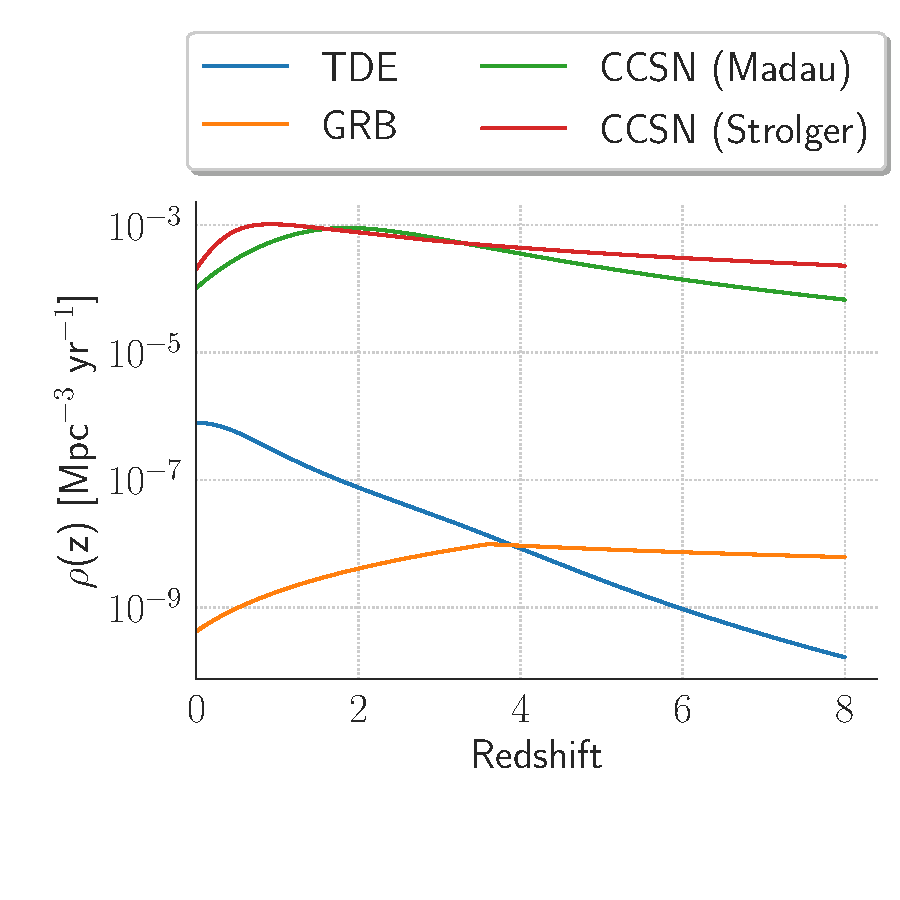
\includegraphics{nu_cosmology/rhoz}
	\caption{Various transient rate densities as a function of redshift.}
	\label{fig:rhoz}
\end{marginfigure}

An alternative driver of evolution is the density of supermassive black holes (SMBHs), which are connected with many other sources such as blazars, radio galaxies and TDEs. In contrast to the SFR, massive SMBHs are thought to be formed through mergers of smaller SMBHs. The density of massive SMBHs thus has a tendency to increase over time, so is higher in the local universe than at more distant redshifts. In contrast to the SFR, the SMBH density thus has a \emph{negative source evolution}. Of particular relevance to this thesis is the rate of TDEs, which have been proposed theoretically to follow this negative SMBH evolution  \sidecite{Sun:2015bda}, as illustrated in Figure \ref{fig:rhoz}. Caution must be taken for this rate, since TDEs are primarily detected in the local universe, so the high-z rates are broadly unconstrained observationally. 

With any chosen source rate/density and neutrino spectrum, we can calculate the corresponding \emph{cumulative neutrino flux} arising from that population \cite{Strotjohann2020Search}. For steady sources, we simply find:

\begin{equation}
\overline{\rho(z)} \equiv \frac{dN(z)}{dV_{C}}
\end{equation}

where $\overline{\rho(z)}$ is the local density per unit comoving volume. We can then integrate over the differential `redshift shell' to calculate $\overline{R(z)}$, the density per unit redshift:

\begin{equation}
\overline{R(z)} \equiv \frac{dN(z)}{dz} = \overline{\rho(z)} \times \frac{dV_{C}}{dz}
\label{eq:steady_rate}
\end{equation}

If we instead consider transient objects, additional cosmological effects start to become relevant. In the following, we denote quantities in the source frame with x', while those at Earth are given as x. It is clear that the number of particles itself must be invariant to the frame, i.e N' = N. However, there is in general a process of \emph{cosmic time dilation}, where the passage of time at the source location, t', is slowed when observed at Earth, t:

\begin{equation}
t = (1+z)t'
\label{eq:t}
\end{equation}

\begin{equation}
\frac{dt'}{dt} = \frac{1}{1+z}
\label{eq:dt}
\end{equation}

For a transient rate density $\rho (z)$ as a function of redshift, we can then calculate the rate of transients per redshift shell. The rate is given per unit time, but the impact of time dilation at higher redshifts suppresses the rate by a factor (1+z). 

\begin{equation}
\rho(z) \equiv \frac{dN(z)}{dV_{C}dt'}
\end{equation}

\begin{equation}
R(z) \equiv \frac{dN(z)}{dtdz} = \rho(z) \times \frac{dV_{C}}{dz} \times \frac{1}{1+z}
\label{eq:transient_rate}
\end{equation}

These are illustrated in Figure \ref{fig:rz}. The differential comoving volume of a redshift shell is derived using the \emph{astropy} package \sidecite{astropy_13}. We can then calculate the transient rate in the universe by integrating to high redshift:

\begin{equation}
R_{all} = \int_{0}^{\infty} R(z) dz
\end{equation}

\begin{marginfigure}
	\centering 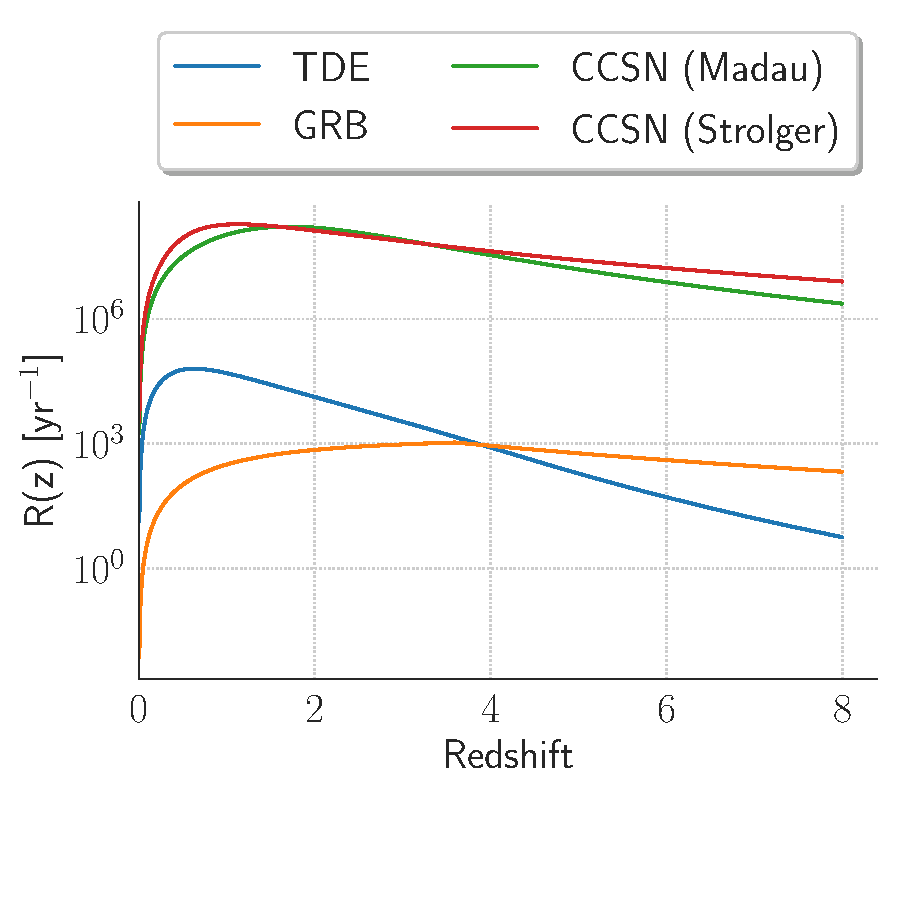
\includegraphics{nu_cosmology/rz}
	\caption{Various transient rates as a function of redshift.}
	\label{fig:rz}
\end{marginfigure}

\section{Differential flux and K-corrections}

Having  calculated the rate of sources, we must next calculate the neutrino flux produced by each individual object. We first consider the isotropic emission of a fixed number of particles, N, by a source. In that case, the particle count per unit area on Earth will ultimately depend only on the \emph{comoving distance} to that object, $D_{c}$:

\begin{equation}
\frac{dN}{dA} = \frac{N}{4 \pi D_{C}^{2}}
\label{eq:particle_per_area}
\end{equation}

If we instead wish to consider the particle flux, we must differentiate this quantity with respect to time:

\begin{equation}
\frac{dN}{dAdt} = \frac{dN}{dt} \times \frac{1}{4 \pi D_{C}^{2}}
\label{eq:particle_flux}
\end{equation}

Often, we only know the emission rate of particles in the source frame, $\frac{dN}{dt'}$, in which case we replace Equation \ref{eq:particle_flux} with:

\begin{equation}
\frac{dN}{dAdt} = \frac{1}{1+z} \times \frac{1}{4 \pi D_{C}^{2}} \times \frac{dN}{dt'}
\label{eq:alt_particle_flux}
\end{equation}

It may be more relevant to consider the luminosity of a source, where the intrinsic source luminosity is defined as:

\begin{equation}
L' \equiv \frac{d}{dt'} \left( \int E' dN \right) = \frac{d}{dt'} \left( \int E' \frac{dN}{dE'} dE' \right)
\end{equation}

However, a second cosmological effect must here be accounted for. The expansion of the universe leads to a process of \emph{redshifting}, so that E', the energy of emitted particles, is not the same as E, the energy at which the particle observed:

\begin{equation}
E = \frac{E'}{1+z}
\label{eq:redshift}
\end{equation}

\begin{equation}
\frac{dE}{dE'} = \frac{1}{1+z}
\label{eq:de}
\end{equation}

We will thus observe a redshifted energy flux, S:

\begin{equation}
S \equiv \frac{d}{dtdA} \left( \int E dN \right) = \frac{1}{1+z} \times \frac{1}{4 \pi D_{C}^{2}} \times \frac{d}{dt'} \left( \int E dN \right)
\end{equation}

\begin{equation}
S = \frac{1}{1+z} \times \frac{1}{4 \pi D_{C}^{2}} \times \frac{d}{dt'} \left( \int E \frac{dN}{dE'} dE' \right)
\end{equation}

\begin{equation}
S = \frac{1}{(1+z)^{2}} \times \frac{1}{4 \pi D_{C}^{2}} \times \frac{d}{dt'} \left( \int E' \frac{dN}{dE'} dE' \right) =  \frac{1}{(1+z)^{2}} \times \frac{L'}{4 \pi D_{C}^{2}}
\label{eq:energy_flux}
\end{equation}

Given the importance of luminosity and energy flux in astronomy, it is conventional to define a new distance measure known as \emph{luminosity distance}, $D_{L}$:

\begin{equation}
D_{L} \equiv \sqrt\frac{L'}{4 \pi S} = D_{C}(1+z)
\end{equation}

In this case, Equation \ref{eq:energy_flux} is reduced to:

\begin{equation}
S = \frac{L'}{4 \pi D_{L}^{2}}
\end{equation}

However, telescopes/detectors are only sensitive in specific energy ranges, so it is typically more important to know the flux at a given energy. This quantity, known as the \emph{differential energy flux}, is defined as:

\begin{equation}
S_{E} \equiv \frac{dS(E)}{dE} = (1+z) \times \frac{dS}{dE'}
\end{equation}

\begin{equation}
S_{E} = (1+z) \times \frac{1}{4 \pi D_{L}^{2}} \times \frac{dL'}{dE'}
\end{equation}
For convenience, we define the \emph{differential luminosity} (or \emph{specific luminosity}):

\begin{equation}
L'_{E'} \equiv  \frac{dL'}{dE'} = \frac{d}{dt'} \left( E' \frac{dN'(E')}{dE'} \right)
\end{equation}

We can then compactly write:

\begin{equation}
S_{E} = (1+z) \times \frac{L'_{E'}}{4 \pi D_{L}^{2}}
\label{eq:kcorrection}
\end{equation}

The above Equation \ref{eq:kcorrection} is the definition of a \emph{k-correction}, a widely-used formula by which the intrinsic source properties of an object can be converted to the expected differential energy flux. This is a generic definition, and is valid for both photon and neutrino fluxes. 

However, for particle detectors such as IceCube, it is instead more common to consider the differential particle flux, given by differentiating Equation \ref{eq:alt_particle_flux}. To conserve particle number despite the impact of redshifting, the observed count rate per unit energy at E, must be equal to the emission rate of particles at energy E':

\begin{equation}
dN(E) = dN'(E')
\end{equation}

\begin{equation}
\frac{dN(E)}{dE} = \frac{dN'(E')}{dE'} \times \frac{dE'}{dE} = (1+z) \times \frac{dN'(E')}{dE'}
\end{equation}

Then we see:

\begin{equation}
\frac{dN}{dAdE dt} = \frac{1}{1+z} \times \frac{1}{4 \pi D_{C}^{2}} \times \frac{dN(E)}{dEdt'}
\end{equation}

\begin{equation}
\frac{dN}{dAdEdt}= \frac{1}{4 \pi D_{C}^{2}} \times \frac{dN'(E')}{dE'dt'}
\end{equation}

For this thesis, it is only relevant to consider the special case where source spectra are power laws with some spectral index, $\gamma$:

\begin{equation}
\frac{dN'(E', t')}{dE'dt'} = \phi_{0}(t') \times \left( \frac{E'}{E_{0}}\right) ^{-\gamma}
\label{eq:def_pl}
\end{equation}

\begin{equation}
L'_{E'}(t') \equiv E' \times \frac{dN'(E', t')}{dE'dt'} = E' \times \phi(t') \times \left( \frac{E'}{E_{0}}\right) ^{-\gamma}
\label{eq:def_le}
\end{equation}

By substituting in Equation \ref{eq:redshift}, we finally reach:

\begin{equation}
\frac{dN(E', t')}{dAdEdt}= (1+z)^{2} \times \frac{1}{4 \pi D_{L}^{2}} \times \phi(t') \times \left( \frac{E'}{E_{0}}\right) ^{-\gamma}
\end{equation}

 \begin{equation}
 \frac{dN(E, t')}{dAdEdt}= (1+z)^{2 - \gamma} \times \frac{1}{4 \pi D_{L}^{2}} \times \phi(t') \times \left( \frac{E}{E_{0}}\right) ^{-\gamma}
 \label{eq:diff_particle_flux}
 \end{equation}
 
Equation \ref{eq:diff_particle_flux} is convenient for steady sources of known luminosity, where $\phi(t') = \phi_{0}$. For transients, it can be more helpful to consider the cumulative time-integrated particle flux per transient. We typically assume a constant flux for a fixed duration $\Delta_{T'} = T'_{1} - T'_{0}$:

 \begin{equation}
\phi(t')  = 
\begin{cases}
\phi_{0} & T'_{0} < t' < T'_{1}\\
0 & otherwise\\
\end{cases}
\end{equation}

\begin{equation}
\int_{0}^{\infty} \phi(t') dt' = \phi_{0} \Delta_{T'}
\end{equation}

We then find:

 \begin{equation}
 \frac{dN(E)}{dAdE} = (1+z)^{2 - \gamma} \times \frac{1}{4 \pi D_{L}^{2}}  \times \left( \frac{E}{E_{0}}\right) ^{-\gamma} \times \int \phi(t') dt 
\end{equation}

 \begin{equation}
\frac{dN(E)}{dAdE}= (1+z)^{3 - \gamma} \times \frac{\phi_{0} \Delta_{T'}}{4 \pi D_{L}^{2}} \times \left( \frac{E}{E_{0}}\right) ^{-\gamma}
\end{equation}
 
\begin{marginfigure}
	\centering \includegraphics{nu_cosmology/dnde}
	\caption{Contributed flux at earth as a function of redshift.}
	\label{fig:dnde}
\end{marginfigure}

Figure \ref{fig:dnde} shows the contributed diffuse flux at Earth as a function of redshift, assuming each transient contributes $10^{50}$ erg distributed in an $E^{-2}$ power law from 1 GeV to 10 PeV. Ultimately, the diffuse flux measured by IceCube will be the integral of this flux-per-source multiplied by the source rate in Equation \ref{eq:transient_rate}:

\begin{equation}
\frac{dN(E)}{dEdAdt} = \int_{0}^{\infty} \left[ \ (1+z)^{2 - \gamma} \times \frac{\rho(z)\phi_{0} \Delta_{T'}}{4 \pi D_{L}^{2}} \times \left( \frac{E}{E_{0}}\right) ^{-\gamma}  \right] \frac{dV_{C}}{dz} dz
\label{eq:nu_flux_tot}
\end{equation}

\begin{marginfigure}
	\centering 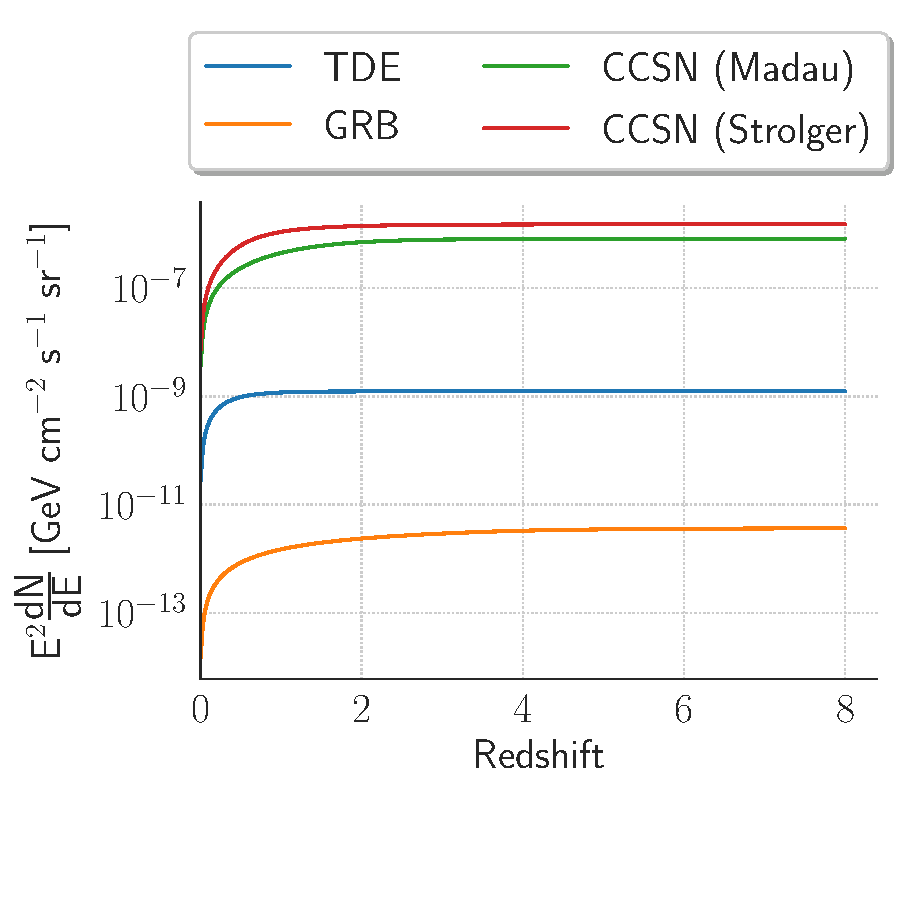
\includegraphics{nu_cosmology/diffuse_flux}
	\caption{Cumulative flux at earth as a function of redshift.}
	\label{fig:diffuse_flux}
\end{marginfigure}

These cumulative neutrino fluxes are shown in Figure \ref{fig:diffuse_flux}. For steady sources, using Equations \ref{eq:steady_rate} and \ref{eq:diff_particle_flux}, we similarly find:

\begin{equation}
\frac{dN(E)}{dEdAdt} = \int_{0}^{\infty} \left[ \ (1+z)^{2 - \gamma} \times \frac{\overline{\rho(z)}\phi_{0}}{4 \pi D_{L}^{2}} \times \left( \frac{E}{E_{0}}\right) ^{-\gamma}  \right] \frac{dV_{C}}{dz} dz
\label{eq:nu_flux_tot_steady}
\end{equation}

\section{Comparing Source Classes}

Equation \ref{eq:nu_flux_tot} reveals differences in the characteristic behaviour of different possible neutrino source populations. The impact of differing the spectral index is illustrated in Figure \ref{fig:CDF_gamma}, using the TDE rate, where softer spectral indices lead to a flux slightly more dominated by nearby sources. Given that high-z transients are already suppressed, the overall impact is relatively minor. However, as is clear in both Figure \ref{fig:dnde} and \ref{fig:CDF_rate}, the source evolution heavily impacts the relative contribution of nearby sources to the diffuse flux. A survey complete up to z=0.25 would already detect sources responsible for 60\% of all TDE neutrino emission, whereas it would contain just 20-25\% of CCSN neutrino emission. Each curve in Figure \ref{fig:CDF_rate} gives the per-neutrino probability of detecting a counterpart as a function of maximum redshift.

\begin{marginfigure}
	\centering 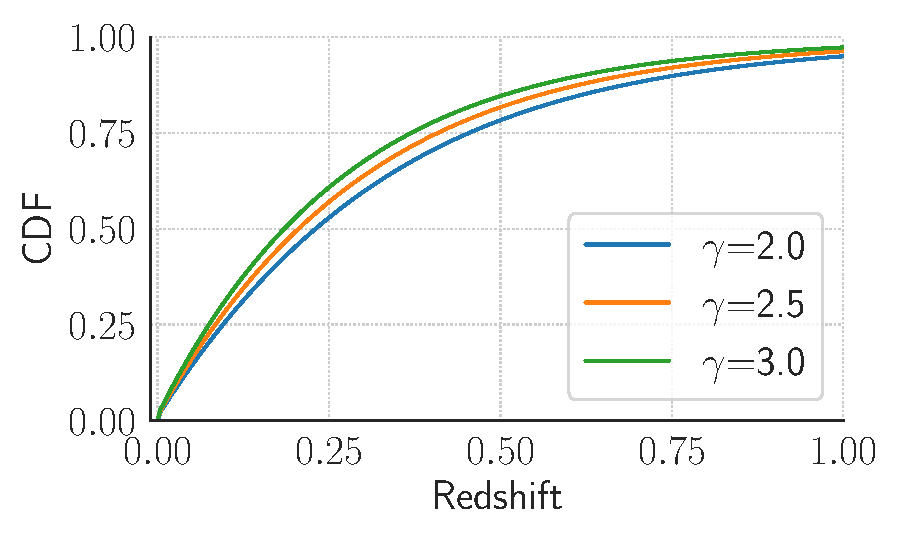
\includegraphics{nu_cosmology/flux_gamma}
	\caption{Neutrino flux CDF as a function of spectral index for TDEs.}
	\label{fig:CDF_gamma}
\end{marginfigure}


\begin{marginfigure}
	\centering 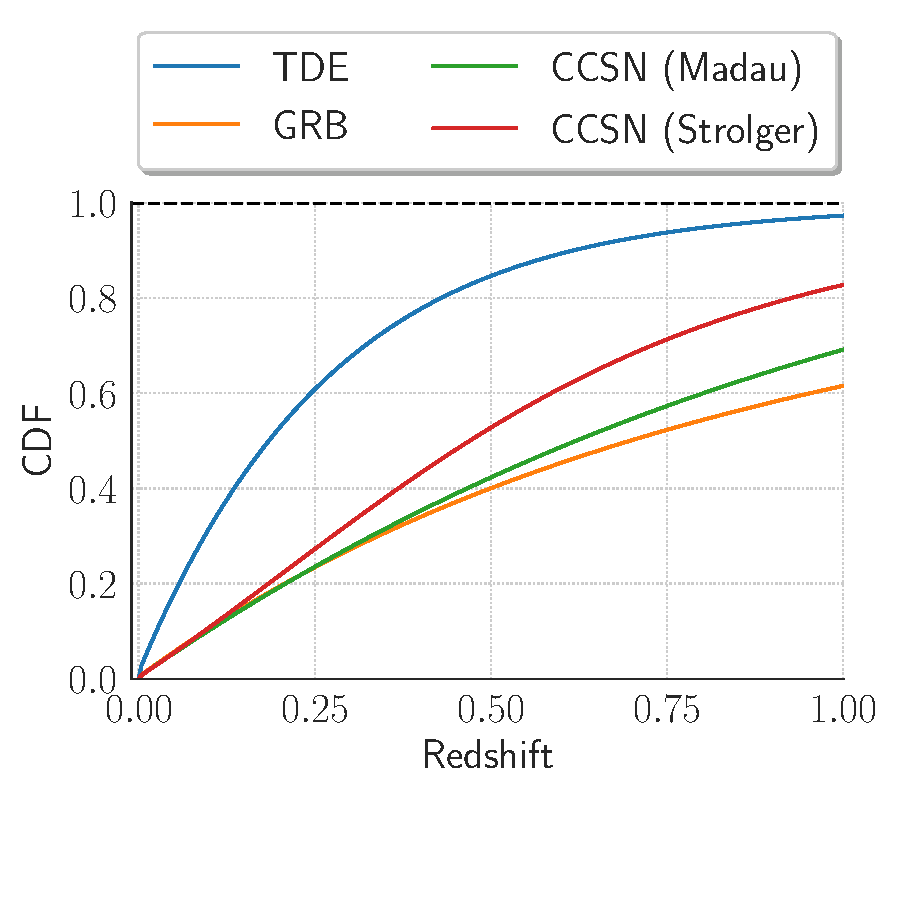
\includegraphics{nu_cosmology/diffuse_flux_rates}
	\caption{Neutrino flux CDF as a function of source evolution.}
	\label{fig:CDF_rate}
\end{marginfigure}

\begin{marginfigure}
	\centering 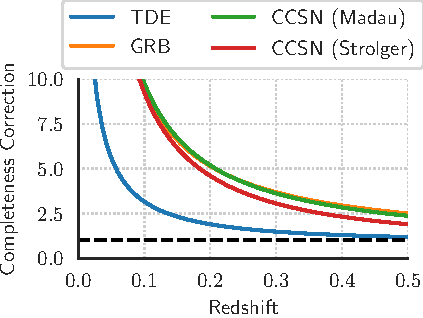
\includegraphics{nu_cosmology/diffuse_flux_completeness}
	\caption{Completeness correction factor as a function of source evolution.}
	\label{fig:completeness}
\end{marginfigure}

Figure \ref{fig:completeness} illustrates the completeness correction factor as a function of redshift. For a sample complete up to a redshift of z, multiplying the sample flux by the correction factor will yield the total population flux. Equivalently,  this factor is the number of population neutrinos that would need to be followed up before one counterpart could be identified, assuming that the follow-up instruments were sensitive up to redshift z. This Figure illustrates most starkly the challenge of optical follow-up of neutrinos, and the relative sensitivity to different source evolutions. For a TDE-like negative rate, the cumulative neutrino flux  will be overwhelmingly dominated by nearby sources, while transients that evolve with the Star Formation Rate (e.g CCSNe) have a much larger contribution from more distant sources.

To give a specific example revisited in Chapter \ref{ch:bran}, ZTF is approximately complete in identifying TDEs up to a redshift of 0.15. Per Figure \ref{fig:CDF_rate}, this volume will contain sources responsible for roughly 40\% of the population flux, so from Figure \ref{fig:completeness}, we see that we would expect to find roughly 2/5 of counterparts to TDE neutrinos. In contrast, CCSNe tend to be dimmer, and with completeness rapidly deteriorating above a redshift of z $\sim$0.05 \sidecite{ztf_bts}. Even neglecting this effect, with SFR-evolution only 12\% of neutrinos will be produced in the volume z<0.15.

To approximately quantify the impact of this effect, we can consider the general power of counting experiments probing this region. The number of signal detections, $N_{sig}$, is proportional to the fraction of flux belonging to resolvable sources, while the rate of background/chance coincidences, $N_{bkg}$, is proportional to the number of sources within this observable volume.

We consider a neutrino with typical properties for those issued as IceCube realtime alerts. We assume it has a \emph{signalness} of 50\%, i.e that it has a 50\% probability to be of astrophysical origin rather than from atmospheric backgrounds. Such alerts are typically reported with a median angular error of $\sim$1 degree. Any source class will then have a cumulative expectation of 0.5 $\times f_{\textup{tot}}$, where $f_{\textup{tot}}$ is the fraction of the total diffuse astrophysical neutrino flux contributed by that source class. 
		
We consider a number of source classes, listed in Table \ref{tab:source_properties}. We calculate their expected background rate by considering their sky rate, given as a product of their local rate, integrated to a typical telescope horizon, and multiplied by a typical telescope detection efficiency. For each source, we also multiply the appropriate search window for neutrino emission, yielding a final background density for any point on the sky. Multiplying this by the neutrino localisation area gives us the ultimate background rate per follow-up. We also consider the expected signal per search, given as the neutrino population expectation multiplied by the fraction of flux which is produced by sources accessible to telescopes. These are illustrated in Figure \ref{fig:nsig_nbkg} for a variety of source classes. Unlike other populations in Table  \ref{tab:source_properties}, GRBs are typically detected with poorly localisation, resulting in a higher background coincident rate.

\begin{table*}[]
	\centering
	\begin{tabular}{||c c c c c c c|} 
	\hline
	Source & Max & Length & Search & Detection & Local & Source \\
	Class & Redshift & &  Area & Efficiency & Rate & Evolution\\
	& [z] & [yr] & [sq. deg.] & [\%] & [Mpc$^{-3}$ yr$^{-1}$] & \\
	\hline
	TDE (Non-jetted) & 0.15 & 1.00 & 3.14 & 100.00 & 8.0$ \times10^{-7}$  & TDE \cite{Sun:2015bda}\\
	TDE (Jetted) & 0.50 & 0.50 & 3.14 & 100.00 & 3.0$ \times10^{-11}$  & TDE \cite{Sun:2015bda}\\
	SN IIP & 0.05 & 0.30 & 3.14 & 100.00 & 5.3$ \times10^{-5}$ & SFR \cite{sfr_madau_14}\\
	SN Ic & 0.05 & 0.03 & 3.14 & 100.00 & 1.8$ \times10^{-5}$  & SFR \cite{sfr_madau_14}\\
	SN IIn & 0.08 & 0.30 & 3.14 & 100.00 & 6.5$ \times10^{-6}$  & SFR \cite{sfr_madau_14}\\
	FBOT & 0.25 & 0.30 & 3.14 & 100.00 & 7.0$ \times10^{-7}$ & SFR \cite{sfr_madau_14}\\
	GRB & 1.00 & 3.2$ \times10^{-6}$ & 314.16 & 100.00 & 4.2$ \times10^{-10}$  & GRB \cite{grb_lien_14} \\
	FRB (complete) & 1.00 & 3.2$ \times10^{-10}$  & 3.14 & 100.00 & 0.072 & SFR \cite{sfr_madau_14}\\
	FRB (0.1\%) & 1.00 & 3.2$ \times10^{-10}$  & 3.14 & 0.10 & 0.072 & SFR \cite{sfr_madau_14} \\
	\hline
	\end{tabular}
	\caption{Summary of assumptions on source classes.}
	\label{tab:source_properties}
\end{table*}{}

\begin{figure}[!ht]
	\centering 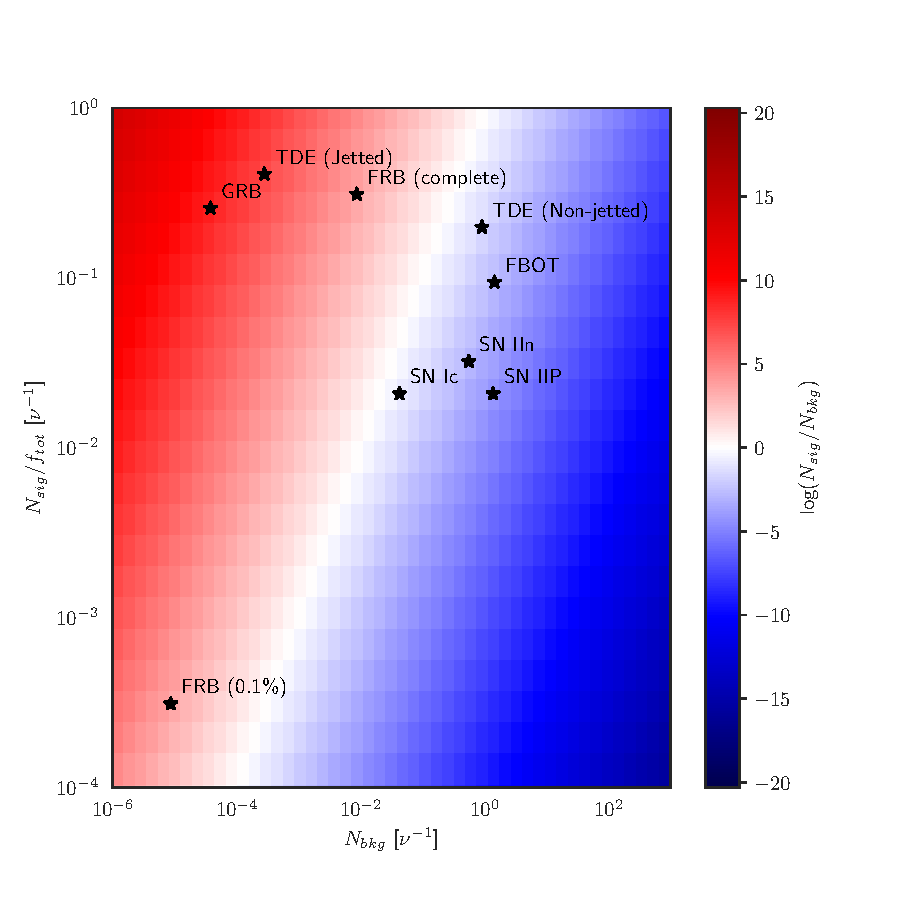
\includegraphics{nu_cosmology/nsig_nbkg}
	\caption{Per neutrino ($\nu^{-1}$) $N_{sig}$ vs $N_{bkg}$ for a variety of source classes.}
	\label{fig:nsig_nbkg}
\end{figure}

The intrinsic signal-to-noise of different source classes can be seen in Figure \ref{fig:nsig_nbkg}, with the white band indicating the transition from the red signal-dominated regions to the blue background-dominated regions. In general, the probability of observing a coincidence increases from the bottom to top, while the significance of any coincidence increases from lower right to upper left. In all cases, the y axis represents the probability of observing a coincidence. For sources with $N_{\textup{bkg}} \lesssim 0.1$, where the probability of multiple background events is negligible, the x axis corresponds to the p-value for a coincidence. Neutrino-specific properties of signalness and localisation will linearly scale all points in the x or y direction respectively, but the relative positions of populations remains unchanged. 

One particularly noteworthy class is FRBs, which should be particularly favourable owing to their extremely stringent temporal localisation. Indeed, were telescopes fully efficient at detecting these across the sky, the limits on this class would be perhaps the most stringent of all. However, at the time of the most recent IceCube analysis, just 21 FRBs were tested against an estimated rate of $\sim$3000 per sky per day, a sample for which no constraint could be placed on the FRB population \sidecite{icrc_frb}. This is a direct consequence of the detection efficiency of FRBs, which is so low that only a tiny fraction of signal is detectable. The expected signal to background ratio for FRBs is very high, and this statement is independent of detection efficiency, so any FRB-neutrino coincidence would be very strong evidence for a physical association. However, because the probability that an FRB counterpart would be detected at all is so low at present, no coincidence is likely to be found. This more realistic scenario is also illustrated in Figure \ref{fig:nsig_nbkg}, where with a more realistic assumed detection efficiency of 0.1\% FRBs illustrates the substantial contrast to other source classes.

We can further quantify how the expected significance would change with increasing numbers of follow-up campaigns for different possible source populations. In a real experiment, integer numbers of counterparts would be detected, for which we could then calculate the poisson probability of chance coincidence, the \emph{p-value} (see Chapter \ref{ch:llh}). This gives us the expected statistical significance of each Nth detection. However, the \emph{regularised lower incomplete Gamma function}, $G (y, \lambda)$, can be used to approximate a continuous poisson distribution \sidecite{incomplete_gamma}:

\begin{equation}
G (y, \lambda) = \int_{\lambda}^{\infty} \frac{t^{y-1} e^{-t}}{\Gamma (y)} dt
\label{eq:incomplete_gamma}
\end{equation}

where ${\Gamma (y)}$ is the gamma function:

\begin{equation}
\Gamma (y) = \int_{0}^{\infty} t^{y-1} e^{-t} dt
\end{equation}

Equation \ref{eq:incomplete_gamma} enables us to visualise a continuous estimate of statistical significance as a function of background rate and expected signal rate. This is shown in Figure \ref{fig:p_value}, using the same assumptions listed in Table \ref{tab:source_properties}, with the p-values converted to Gaussian $\sigma$ values. The starting x position of each curve indicates how many detections would be needed before one counterpart was detected, while the y position quantifies the statistical significance of this first signal detection given the background rate. The remainder of the curve shows how this statistical significance might be expected to evolve as a function of the number of follow-up campaigns, $N_{followup}$.

\begin{figure}[!ht]
	\centering 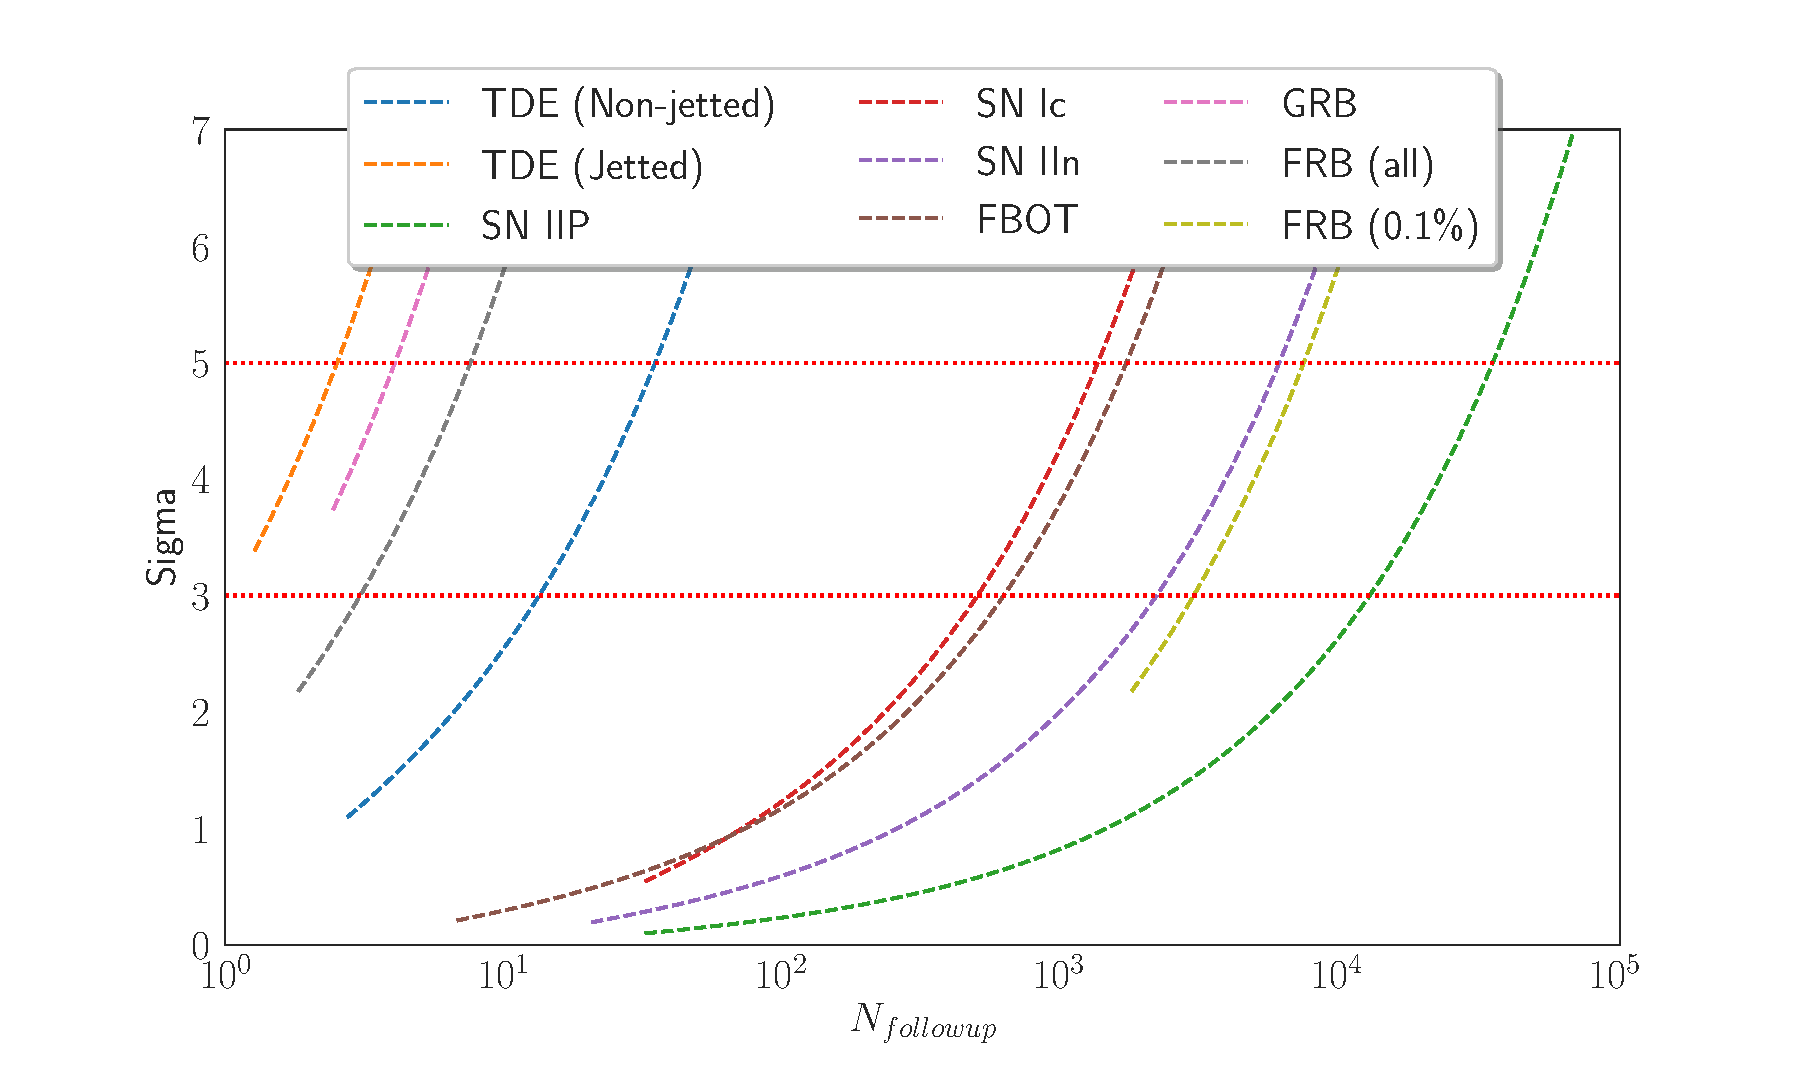
\includegraphics{nu_cosmology/p_value_nfollowup}
	\caption{Statistical significance of excess coincidence as a function of number of follow-ups.}
	\label{fig:p_value}
\end{figure}

As a lower detection efficiency will decrease the signal detection rate,  it will be represented in Figure \ref{fig:p_value} as a shift of a curve to the right,  as can be seen for the two FRB curves. However, because the background rate is also reduced proportionately, the y axis remains unaffected. In other words, with lower detection efficiency one must do more follow up campaigns to detect N coincidence, but the significance of each nth coincidence found is independent of detection efficiency.

It should be noted that the results presented in Figure \ref{fig:p_value} implicitly assume that each detected object is equally likely to be a neutrino counterpart, and are thus analogous to a so-called \emph{equal weighting} scenario as introduced in Equation \ref{eq:equal_weighting} of Chapter \ref{ch:llh}. However, rather than such a simple counting experiment, it is typical to incorporate additional information in a likelihood analysis which weight the probability for each potential counterpart. One example would be to assume neutrino emission is proportional to inverse square of luminosity distance, or to flux/fluence at a particular energy band, or correlated to a particular subclass of a population. If any such additional information is used, further background discrimination will be possible, leading to higher significance correlations for fixed $N_{followup}$. Figure \ref{fig:p_value} thus provides a lower limit on the power of any follow-up campaign targeting any source class with the properties introduced in Table \ref{tab:source_properties}. The curves do not directly depend on the observation band of a given instrument, but the individual telescope characteristics will alter the typical detection efficiency/maximum redshift. 

Though Figure \ref{fig:p_value} contains no analysis of IceCube data, it is particularly notable that the position of sources correspond closely to the relative constraints that have been placed on those classes by IceCube (see Table \ref{tab:source_limits} of Chapter \ref{ch:sources}). Those sources near the left of Figure \ref{fig:p_value} are those with the strictest existing limits, often at percent-level, while those nearer the right portion are only weakly constrained or could still produce the entire diffuse flux. The plot illustrates how well the full unbinned likelihood analysis method used by IceCube for neutrino astronomy can, to first order, be approximated by a poisson counting experiment. Those source classes on the left (TDEs, GRBs, FRBs with high detection efficiency) are those most favourable for detection with realtime follow-up programs such as the one introduced in Chapters \ref{ch:realtime} and \ref{ch:ztf}. 
